\section{Joint versus Independent Framework for Supervised Cross-modal Retrieval}
\label{sec:LMI}

Researchers in academia and industry have begun focusing on cross-modal retrieval due to the rapid increase in multimodal data, such as images, text, audio, video, and so on. Interestingly, this multimodal data can be obtained from a single source or multiple sources simultaneously or at varying time intervals. However, most existing cross-modal retrieval approaches \cite{dwijesh, clip4cmr, dscmr} jointly learn a common representation space, facing the following three disadvantages:
1) \textbf{Scalable multimodal learning}: The majority of methods are designed for two modalities, and they require \(\frac{m(m - 1)}{2}\) iterations for \(m\) modalities (typically m > 2) in a pairwise manner, which is time-consuming for multimodal datasets. 
2) \textbf{Adding new modality data:} Most of the methods require retraining the entire model for the new modality, as the training process requires the presence of data from all modalities.
3) \textbf{Computational resources:} Jointly training data from all the modalities requires a large number of computational resources, like storage. 

\par To solve these disadvantages, we propose a \textit{Lightweight Modality-Independent Framework (LM-I)} for \textit{supervised cross-modal retrieval} and explore if achieving effective retrieval without learning a common representation space is possible.
LM-I learns a lightweight linear transformation of each modality into an independent but semantically similar label space. It utilizes a shallow feed-forward network for each modality to transform input embeddings and their respective auto-encoders to project class labels into a modality-independent representation space. It is scalable in terms of computational resources as different modalities can be trained independently and require linear time to train \(m\) modalities.
For inference, we use our \textit{2-stage k-nearest neighbor (2Sknn) search} algorithm, introduced in chapter \ref{sec:lcm} for retrieval.

\begin{figure*}[htbp]
    \centering
    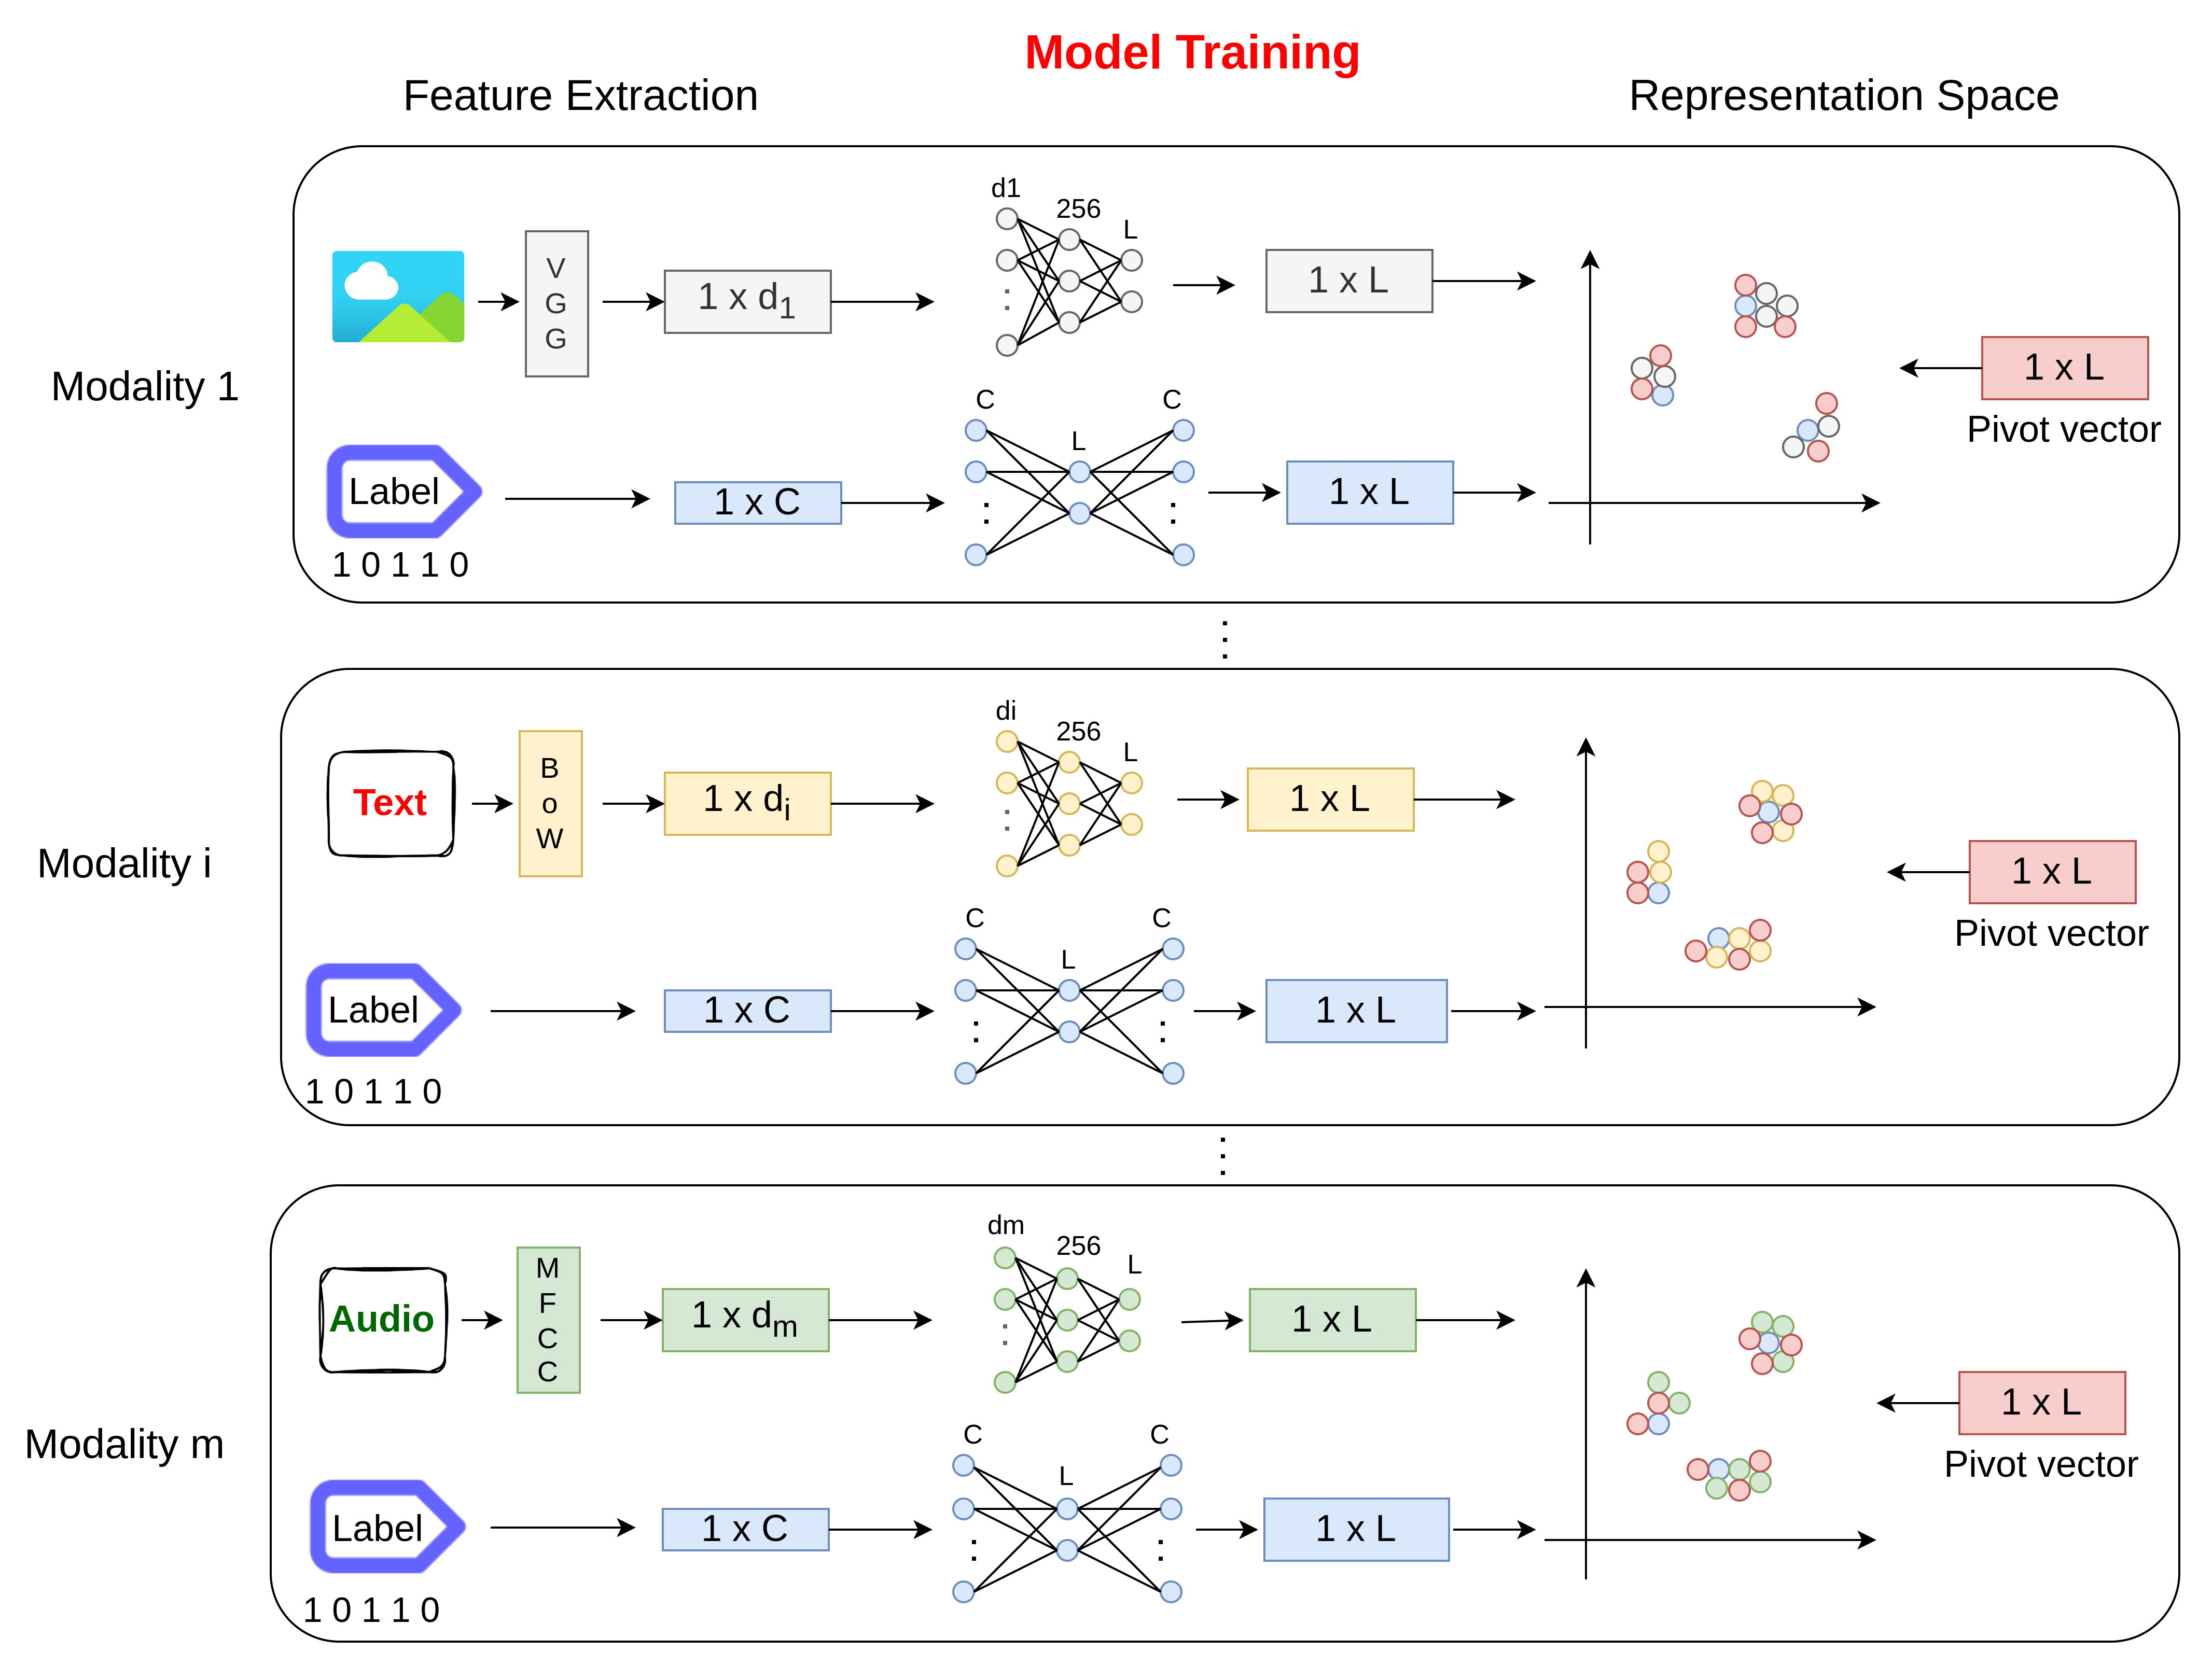
\includegraphics[width=\textwidth]{Figures/lmi.png}
    \caption{Model Training for LM-I.}
    \label{fig:lmi_training}
\end{figure*}

\subsection{Related Work}
Numerous hashing and real-valued techniques for cross-modal retrieval have been proposed in the literature \cite{djsrh, ocmfh, acmr, dscmr}. The key idea in these methods is to first learn a common space shared by different modalities, either independently or in a joint manner, and then use the hamming distance or cosine distance to measure the similarity between items from different modalities. The objective of Scalable Deep Multimodal Learning for Cross-Modal Retrieval (SDML) \cite{sdml} is to learn the transform functions that can project the data of different modalities into a predefined common subspace, in which the between-class variation is maximized while the within-class variation is minimized. It is scalable, as each modality has its own independent parameters that can be learned in parallel. The Separated Variational Hashing Networks for Cross-Modal Retrieval (SVHN) \cite{svhn} initially trains a label network (LabNet) to produce distinct hash codes. Subsequently, modality-specific variational networks (MVNs) are trained to ensure that the latent variables closely approximate the hash codes generated by LabNet while also being constrained by a prior distribution. Furthermore, this method is scalable since each MVN can be trained independently. It is also efficient, as it can convert various modalities into a shared Hamming space using only one program execution. The Decoupled CVH Network (DCHN) \cite{joint} initially generates a hash code by training a semantic hashing auto-encoder module (SHAM) using a few labels or only the number of categories as inputs. This hash code is then utilized to train the view-specific multiview hashing networks (MHNs). In contrast to our approach, all the scalable modality-independent multimodal learning methods project the data from multiple modalities into a single shared common space. However, our LM-I method learns independent modality-specific representation spaces that are discriminated using the label data. LM-I utilizes FAISS, a highly scalable nearest-neighbor indexing technique, and employs 2Sknn for ranking and retrieval tasks.

\subsection{Proposed Framework}
The LM-I framework consists of two parts: model training and 2Sknn retrieval. In model training, as shown in Figure \ref{fig:lmi_training}, we project modality \(m\) using a feed-forward neural network and labels using an auto-encoder network onto a modality-specific representation space. We attempt to minimize the distance between similar items and their labels using projection loss, auto-encoder loss, and pivot loss in this space. The pseudocode of the model training process of $i^{th}$ modality is given in Algorithm~\ref{alg:training}. At inference time, we project the query into the modality-specific representation space, locate nearest neighbors in the same modality, rank labels according to their frequency, and sort cross-modal items for recommendation using the 2Sknn algorithm. 

\begin{algorithm}[htbp]
% \scriptsize
\caption{Model Training of $i^{th}$ modality}
\label{alg:training}
\begin{algorithmic}[1]
    \State \textbf{Task:} Model training
    \State \textbf{Input:} $X_{i}, Y$
    \State \textbf{Output:} Learn deep neural models $F$
    \State Normalize $X_{i}$
    % \mathcal{L}_{intra} = \mathcal{L}_{rec} + \sigma\mathcal{L}_{latent}
    % \While{($loss_{1}+loss_{2}+loss_{3}+loss_{4}$) not converged}
    \While{($\mathcal{L}_{F} + \mathcal{L}_{intra}+\mathcal{L}_{pivot}$) not converged}
        \State $\mathcal{L}_{F}$ = train $i^{th}$ modality projection model: $F_i$
        \State $\mathcal{L}_{intra}$ = train $i^{th}$ modality autoencoder network for label projection
        % \State \Comment{Steps 6, 7, 8 can be implemented in parallel}
        \State $\mathcal{L}_{pivot}$ = update $i^{th}$ modality pivot matrix $B_i$
    \EndWhile
    \State \Return $F_i$
\end{algorithmic}
\end{algorithm}

\subsection{Experimental Setup}
\noindent\textbf{Datasets and Features: }To verify the efficacy of our proposed approach, we conduct experiments on both uni-labeled and multi-labeled datasets. The PKU Xmedia dataset is a multimodal uni-labeled benchmark consisting of 5000 images, 5000 texts, and 1000 audio samples represented using VGG, BoW, and MFCC features provided with \cite{xmedianet, JRL} respectively. The different modalities in the dataset are obtained from different sources through web crawling. The images are obtained by crawling from Flickr, the text is sourced from Wikipedia, and the audio is acquired from the Freesound website. The dataset is divided into 20 distinct categories, namely insect, bird, wind, dog, tiger, explosion, elephant, flute, airplane, drum, train, laughter, wolf, thunder, horse, autobike, gun, stream, piano, and violin. Each text is a paragraph of an article about the category in Wikipedia and most of the texts are less than 200 words. The images are pictures with high resolution which contain the object of each category. The collected audio clips are mostly shorter than one minute. We also curated our own multimodal, multi-labeled dataset using Wikipedia, consisting of modalities like image, text, and structured tabular data. We randomly chose a subset of data items from the WikiTables dataset \cite{wikitables} and used their wiki entities to crawl the associated aligned image and text data. This dataset contains 13962 samples of each modality. We used CLIP features to represent images and text. We experimented with representing the table as a linearized text using CLIP features and as a table using TaPas \cite{tapas} features. We labeled our dataset using YAGO-3 (WordNet-version) into 150 categories, namely award, commissioner, overview, scholar, dancer, cricketer, convert, missionary, scientist, poet, guitarist, count, comedian, contestant, rival, boxer, venue, doctor, princess, composer, official, presenter, king, lieutenant, peer, legislator, location, commune, organization, school, electorate, skater, era, participant, image, journalist, contest, feature, pitcher, vehicle, screenwriter, manufacturer, railway, militant, opera, academician, model, athlete, constituency, sheriff, duke, representative, building, defender, airport, admiral, county, ruler, company, car, champion, executive, cardinal, earl, speaker, senator, archbishop, soldier, event, ballplayer, district, forward, baronet, village, companion, baron, discography, municipality, datum, ambassador, secretary, woman, colleague, diplomat, expressway, knight, season, area, director, prosecutor, road, emigrant, driver, bishop, exile, medalist, coach, sovereign, musician, leader, writer, actress, governor, general, report, race, president, singer, mayor, judge, minister, person, town, artist, actor, university, station, congressman, officeholder, lawyer, player, politician, city, site, alumnus, football coach, baseball coach, basketball coach, volcanic crater, film director, administrative district, lieutenant governor, senior high school, educational institution, filmmaker, council member, foreign minister, commanding officer, army officer, military officer, musical organization, soccer player, tennis player, hockey player, basketball player, football player, county seat, state senator, railway station, military unit. Each text is a paragraph of an article about the Wikipedia entity. The images are the \textit{pageimage} of the Wikipedia entity in high resolution. The structured table is the WikiTable about the Wikipedia entity.

\noindent\textbf{Evaluation Metrics: }For comparison with the baseline, we used mAP and nDCG as metrics. For nDCG, relevance score = |overlapping labels | / |union of labels in q and retrieved item| 

% In the class distribution shown in the figure, we noticed that "person" was the most common class. We then kept the "person" class with data samples that only had the "person" class and no other classes.

% \begin{figure*}[h]
%     \centering
%     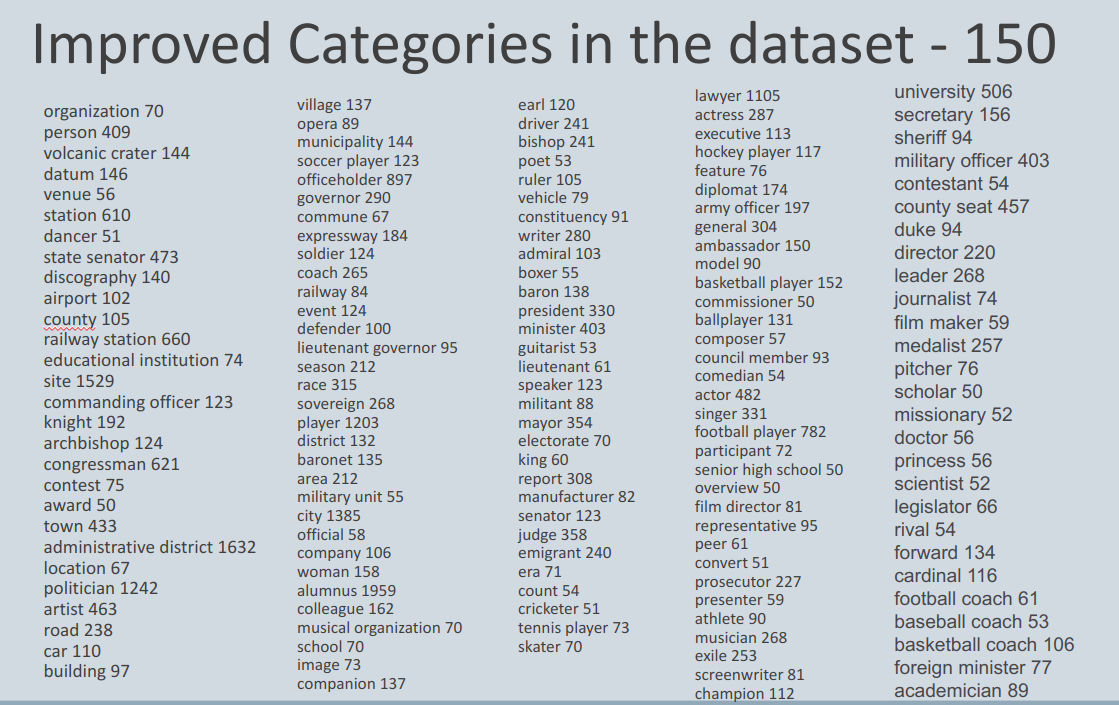
\includegraphics[width=\textwidth]{Figures/dataset.png}
%     \caption{Distribution of classes in our curated dataset.}
%     \label{fig:lmi_training}
% \end{figure*}
\subsection{Experimental Results}
In Table \ref{tab:lmi}, we compare our LM-I with the existing SOTA method DCHN \cite{joint} to demonstrate the efficacy of our proposed method. Note that we cannot compare fairly with LCM as the Xmedia dataset does not have directly aligned data samples; thus, learning the common representation with uneven modality samples is unfair. Table \ref{tab:lmi_our} compares our joint framework LCM with our independent framework LM-I on our curated multimodal dataset using mAP and nDCG metrics. We can note that the LM-I significantly outperforms the existing baselines, and the results of both LCM and LM-I only depend upon the modality of the input query. 

\begin{table}[htbp]
\centering
\caption{\textbf{Comparison of LM-I with a baseline on Xmedia dataset using mAP. Here, L is the length of hash codes for DCHN and the length of embeddings for LM-I}}
\label{tab:lmi}
\resizebox{\textwidth}{!}{%
\begin{tabular}{@{}c|c|cc|cc|cc|c@{}}
\toprule
Model        & L   & I-T   & I-A   & T-I   & T-A   & A-I   & A-T   & Total Training Time (sec) \\ \midrule
DCHN         & 32  & 88.9  & 87.9  & 92.1  & 89.5  & 45.1  & 45.1  & 264.833                   \\
DCHN         & 64  & 88.8  & 84.7  & 89.4  & 83.1  & 42.9  & 42.9  & 275.845                   \\
DCHN         & 128 & 88.6  & 82.4  & 90.3  & 79.2  & 41.8  & 41.3  & 270.471                   \\ \midrule
% LCM & 32  &  &  &  &  &  &  & \\
% LCM & 64  &  &  &  &  &  &  & \\
% LCM & 128 &  &  &  &  &  &  & \\ \midrule
LM-I + 2Sknn & 32  & 92.15 & 92.15 & 94.79 & 94.79 & 64.15 & 64.15 & 106.441  \\
LM-I + 2Sknn & 64  & \textbf{92.63} & \textbf{92.63} & 95.76 & 95.76 & 65.75 & 65.75 & 94.02 \\
LM-I + 2Sknn & 128 & 92.54 & 92.54 & \textbf{95.79} & \textbf{95.79} & \textbf{68.3}  & \textbf{68.3 } & 90.35 \\ \bottomrule
\end{tabular}%
}
\end{table}
 
\begin{table}[htbp]
\centering
\caption{\textbf{Comparison of LM-I with LCM method on our curated Wikipedia dataset}}
\label{tab:lmi_our}
\resizebox{\textwidth}{!}{%
\begin{tabular}{@{}c|c|c|c|ccc|ccc@{}}
\toprule
\multirow{2}{*}{Model} &
  \multirow{2}{*}{\begin{tabular}[c]{@{}c@{}}Image \\ Features\end{tabular}} &
  \multirow{2}{*}{\begin{tabular}[c]{@{}c@{}}Text \\ Features\end{tabular}} &
  \multirow{2}{*}{\begin{tabular}[c]{@{}c@{}}Table \\ Features\end{tabular}} &
  \multicolumn{3}{c}{mAP} &
  \multicolumn{3}{c}{nDCG@100}  \\
  &      &      &       & Image to any & Text to any & Table to any & Image to any & Text to any & Table to any \\ \midrule
% LCM  & clip & bert & clip  & 66.87 & 77.69 & 72.77 & 85.55 & 86.68 & 86.40 \\
LCM  & clip & clip & tapas & 78.90 & 86.65 & 78.89 & 86.90 & 88.49 & 86.79 \\
LCM & clip & clip & clip & 67.65 & 78.90 & 73.36 & 85.80 & 87.95 & 86.45 \\\midrule
% LM-I & clip & bert & clip  & 80.85 & 78.08 & 83.26 & 93.96 & 93.63 & 94.25 \\
LM-I & clip & clip & tapas & 80.08 & 86.69 & 78.15 & 93.83 & 95.21 & 93.85 \\
LM-I & clip & clip & clip & \textbf{80.85} & \textbf{87.49} & \textbf{83.26} & \textbf{93.96} & \textbf{95.18} & \textbf{94.25}
\\ \bottomrule
\end{tabular}%
}
\end{table}

\subsection{Conclusion}
In this work, we compare the joint versus independent frameworks for supervised cross-modal retrieval. We proposed a Lightweight Modality-Independent Framework for Cross-Modal Retrieval called LM-I, which outperforms the joint framework on our curated multimodal dataset and outperforms the state-of-the-art independent method on the benchmark dataset. 